\documentclass{article}
\usepackage{graphicx}
\usepackage{float}
\usepackage{booktabs}
\usepackage{siunitx}
\usepackage[fleqn]{amsmath}


\title{Lab 2: Getting started with Ohm's Law, KVL, KCL, and Multi-Meter
Measurements}
\author{Sean Balbale}
\date{September 9th, 2023}
\setlength{\parindent}{0in}

\begin{document}

\begin{titlepage}
	\begin{center}
		\vspace*{1in}

		\Huge
		\textbf{Lab 4}

		\LARGE
		Basics of Signals: Frequency

		\vspace{3 in}

		\textbf{Student Name:} Sean Balbale
		\\ \textbf{Instructor:} Dr. Iman Salama
		\\ \textbf{Lab Partner Name:} Krish Gupta
		\\ \textbf{Date:} October 4, 2024

		\vfill


	\end{center}
\end{titlepage}

\newpage


\section{Introduction}
The purpose of this lab was to explore fundamental concepts related to signals,
focusing on their frequency components and behavior. Signals, particularly in
electrical and computer engineering, represent various physical phenomena such
as voltage, current, pressure, sound, or temperature. Engineers often use
sensors and transducers to convert these signals into electrical formats for
analysis and manipulation.
\newline

The lab introduced the use of oscilloscopes and function generators to examine
signals in the time domain. The first part of the lab involved setting up a
function generator to produce different waveforms, such as sinusoidal, square,
and ramp waves, and using an oscilloscope to measure the amplitude, period, and
frequency of these signals. Additionally, an audio speaker was driven by these
waveforms to observe how changes in signal frequency and amplitude affected the
sound produced.
\newline

In the second part of the lab, LTSpice was used to perform transient and
Fourier analysis of circuits with periodic signals. Fourier analysis was
conducted to break down complex waveforms into their frequency components,
helping to visualize the harmonic content of the signals. Different circuit
configurations and signal types were simulated, and the frequency responses were
compared.
\newline

The primary objective was to understand how signals behave in different domains,
both experimentally and through simulation, and how they can be analyzed using
Fourier transformations to reveal their frequency components. This lab formed
the foundation for further studies on signal processing and its applications in
real-world systems.

\section{Results}
\subsection{Frequency}
When the fuction generator was set to produce a 600 Hz sine wave with a 0.10 volt peak to peak 
amplitude, the oscilloscope displayed the same waveform. So the oscilloscope and the function generator agreed.
\newline

The function generator was then hooked up to a speaker which played a 600 Hz tone. The tone changed aas the frequency and
amplitude of the signal changed. The tone was louder when the amplitude was increased and the pitch was higher when the frequency was increased.
\newline
\begin{table}[H]
    \centering
    \begin{tabular}{|c|c|c|}
        \hline
         & Sean & Krish\\
        \hline
        Lower & 30 Hz & 30 Hz \\
        \hline
        Upper & 18.5 kHz & 16 kHz \\
        \hline
    \end{tabular}
    \caption{Hearing Range}
    \label{tab:1.2 hearing range}
\end{table}

As seen in Table ~\ref{tab:1.2 hearing range} We were able to hear close to the 20 Hz to 20 kHz range of human hearing. 
The differences in the range that was percieved could be due to the speaker not being able to produce the full range of 
frequencies or the human ear not being able to hear the full range of frequencies. The as the frequency of the sound 
increaded the pitch and volume of the sound increased.

\begin{figure}[H]
	\centering
	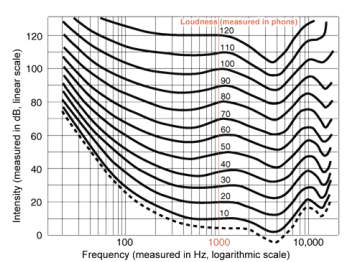
\includegraphics[width=0.5\textwidth]{frequencytointensity.png}
	\caption{Human Hearing Sensitivity}
	\label{fig:fig1}
\end{figure}

This relationship can been seen in Figure~\ref{fig:fig1} which shows the relationship between frequency and intensity of sound.
As the frequency got to the ends of the percievable range the volume of the sound decreased.
\newline

Next we partnered with another group and the function generator was used to produce a sine wave with an unknown frequency.
Using another function generator we tried to match the frequency of the unknown signal by ear. We were able to get within 1 Hz of the
frequency of the unknown signal. This shows that the human ear is able to detect small changes in frequency.
\newline

The function generator was then used top produce 600 Hz sine, ramp, and square waves. The ramp wave was higher pitched and louder than the sine wave.
The square wave was the loudest and highest pitched of the three. This shows that the shape of the wave affects the sound produced.
This is because more time is spent at higher frequencies in the square wave than the sine wave. This is why 
the square wave is louder and higher pitched. the ramp wave is louder and higher pitched than the sine wave because the 
the most time is spent at the highest frequency in the ramp wave. We see the same relationship between the three waveforms when using
a 6 kHz frequency.
\newline

\subsection{LTSpice, Transient and Fourier Analysis}
\begin{figure}[H]
	\centering
	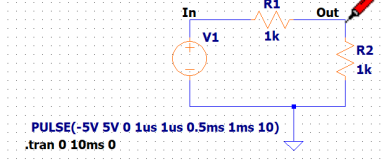
\includegraphics[width=0.5\textwidth]{21Circuit.png}
	\caption{Pulse Circuit}
	\label{fig:fig2}
\end{figure}

In this section of the lab, a transient analysis was performed to observe the
behavior of the voltage across a resistor $R_2$
as a function of time in a given circuit (Figure \ref{fig:fig2}). The transient analysis allowed for the
examination of how the voltage changes over a short time period, particularly
during the application of a periodic input signal. 
\newline

To start, the voltage across $R_1$ was measured using differential probes. One
probe was placed at each end of the resistor to display the voltage difference.
The input signal used had a frequency of 1000 Hz, which corresponds to a period
of 1 millisecond. The total analysis time covered 10 cycles of the waveform,
equating to 10 milliseconds. 
\newline

After plotting the voltage across $R_2$, a Fast Fourier Transform (FFT) was performed on the
output signal to observe its frequency components. FFT is useful for converting
the time-domain signal into the frequency domain, which reveals the individual
frequencies that make up the waveform. This was done by accessing the waveform
viewer window, where the FFT function was selected. 
\newline

Once the FFT was displayed,
the horizontal frequency axis was adjusted by disabling the logarithmic scale
and setting the start frequency at 0 Hz, the end frequency at 30 kHz, and the
step size at 1 kHz. The vertical axis for the magnitude was adjusted to display
in decibels (dB) with the top level set at 20 dB, the bottom level at -50 dB,
and steps of 10 dB. 
\newline

It is important to note that any periodic signal, aside from
a pure sine wave, contains frequencies at multiples (harmonics) of its
fundamental frequency. The FFT revealed these harmonics, showing the frequency
components present in the signal. For example, a square wave contains
significant harmonic content at odd multiples of the fundamental frequency,
unlike a sine wave, which only contains its fundamental frequency. 
\newline 

\begin{figure}[H]
	\centering
	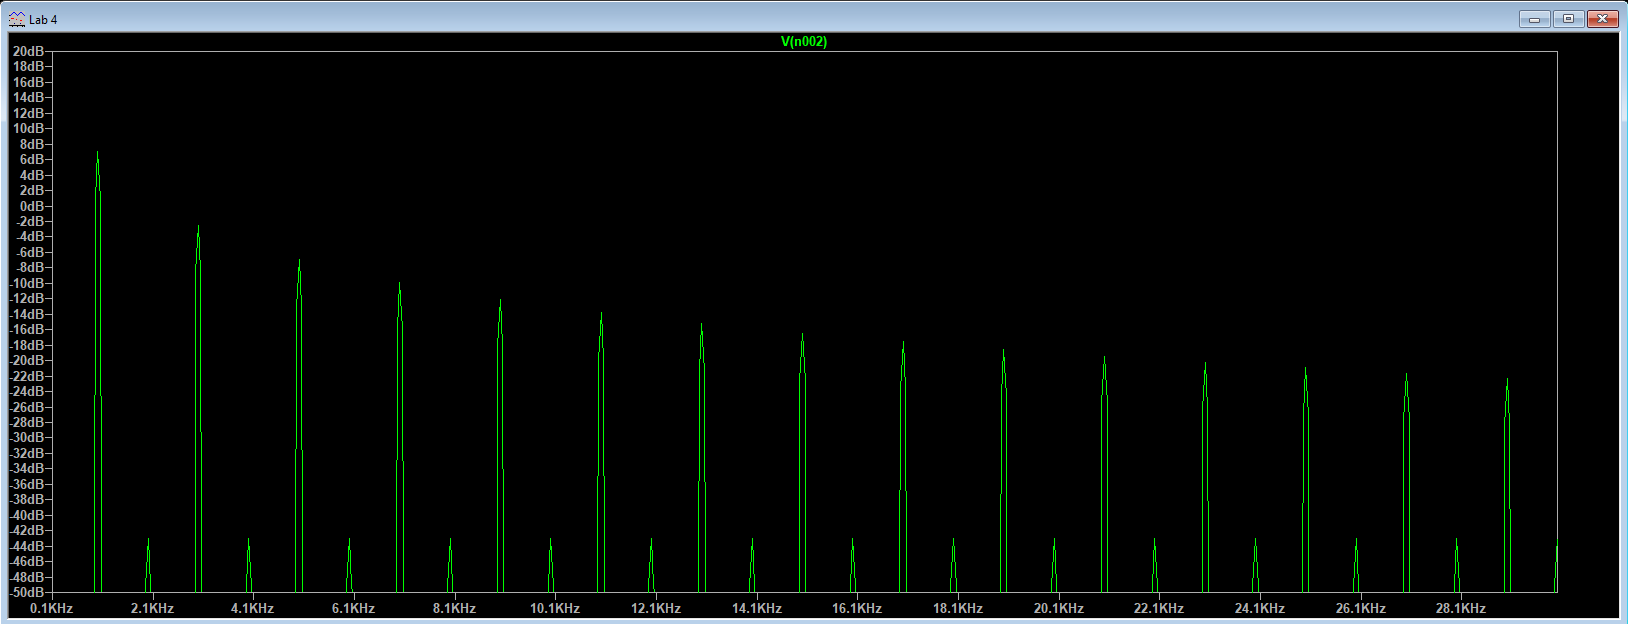
\includegraphics[width=0.75\textwidth]{Copy of Lab 4 - 2.2.PNG}
	\caption{2.2 Pulse FFT}
	\label{fig:fig3}
\end{figure}


The FFT plot can be seen in Figure \ref{fig:fig3}, which shows the frequency components of the pulse waveform. The plot
displays the magnitude of the frequency components in decibels (dB) against the
frequency in kilohertz (kHz). The harmonics of the waveform are visible as peaks
at multiples of the fundamental frequency. The FFT plot provides insight into
the harmonic content of the signal, which is essential for understanding the
frequency composition of complex waveforms. This plot shows the highest intensity at roughly 1 kHz, 
corresponding to the fundamental frequency of the input signal. 
The harmonics are also visible at 3 kHz, 5 kHz, and 7 kHz (this pattern continues to at least 31 kHz), which are the odd 
multiples of the fundamental frequency. This demonstrates the presence of harmonic content in 
the pulse waveform, which is typical for non-sinusoidal signals. The intensity of the harmonics decreases as the frequency increases.
\newline

After repeating the transient analysis with the pulse width $T_on$
set to 0.05 ms, a noticeable change occurred in the frequency components
observed in the Fast Fourier Transform (FFT) plot. By reducing the pulse width,
the signal's duty cycle was decreased, meaning that the time the pulse remains
at its peak voltage ($V_2$) became shorter compared to the total period of the signal.

\begin{figure}[H]
	\centering
	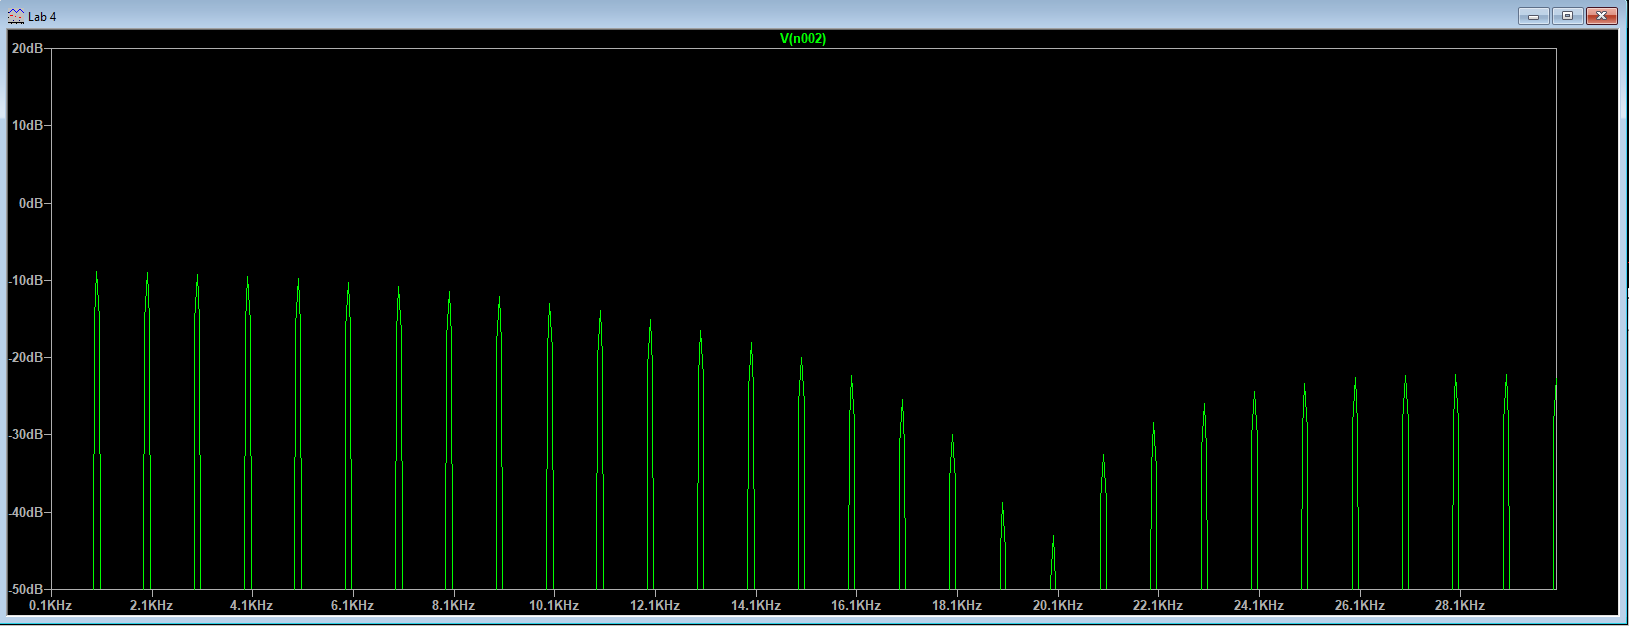
\includegraphics[width=0.75\textwidth]{Copy of Lab 4 - 2.3.PNG}
	\caption{2.3 Pulse FFT}
	\label{fig:fig4}
\end{figure}


This resulted in the lowest strength of the frequency components at 20.1 kHz, which
can been seen in Figure \ref{fig:fig4}. The harmonics at 3 kHz, 5 kHz, and 7 kHz were still present, but their 
intensity was reduced compared to the previous FFT plot. This change in the frequency components
demonstrates how the pulse width and duty cycle of a signal can affect its
harmonic content. 
\newline

When the source was changed to a sinusoidal waveform with a 5 V amplitude, a frequency of 1000 Hz, and all other parameters 
set to zero, the transient analysis was repeated, and the resulting Fast Fourier Transform (FFT) plot showed a significant 
difference compared to the previous analysis with the pulse source.
\newline

Unlike a pulse wave, which contains multiple harmonics, a pure sinusoidal waveform only contains a single frequency 
component—its fundamental frequency. In this case, since the sinusoidal signal had a frequency of 1000 Hz, the FFT 
plot displayed a single dominant peak at 1000 Hz, corresponding to the fundamental frequency of the sinusoidal source.
\newline

No other frequency components (harmonics) were present in the FFT plot, which contrasts with the pulse waveform that 
exhibited higher harmonics at multiples of the fundamental frequency. The absence of harmonics in the sinusoidal 
waveform is because a pure sine wave is considered the simplest periodic signal, containing only its fundamental 
frequency and no additional harmonic content.
\newline

Using the same horizontal axis settings (0 Hz to 30 kHz) and vertical scale (from -50 dB to 20 dB), the FFT plot 
confirmed this result by showing a single peak at 1000 Hz and no significant energy at other frequencies. This outcome 
demonstrates that the sinusoidal waveform, unlike the pulse waveform, does not generate harmonics and therefore has a 
much simpler frequency spectrum.
\newline

\begin{figure}[H]
	\centering
	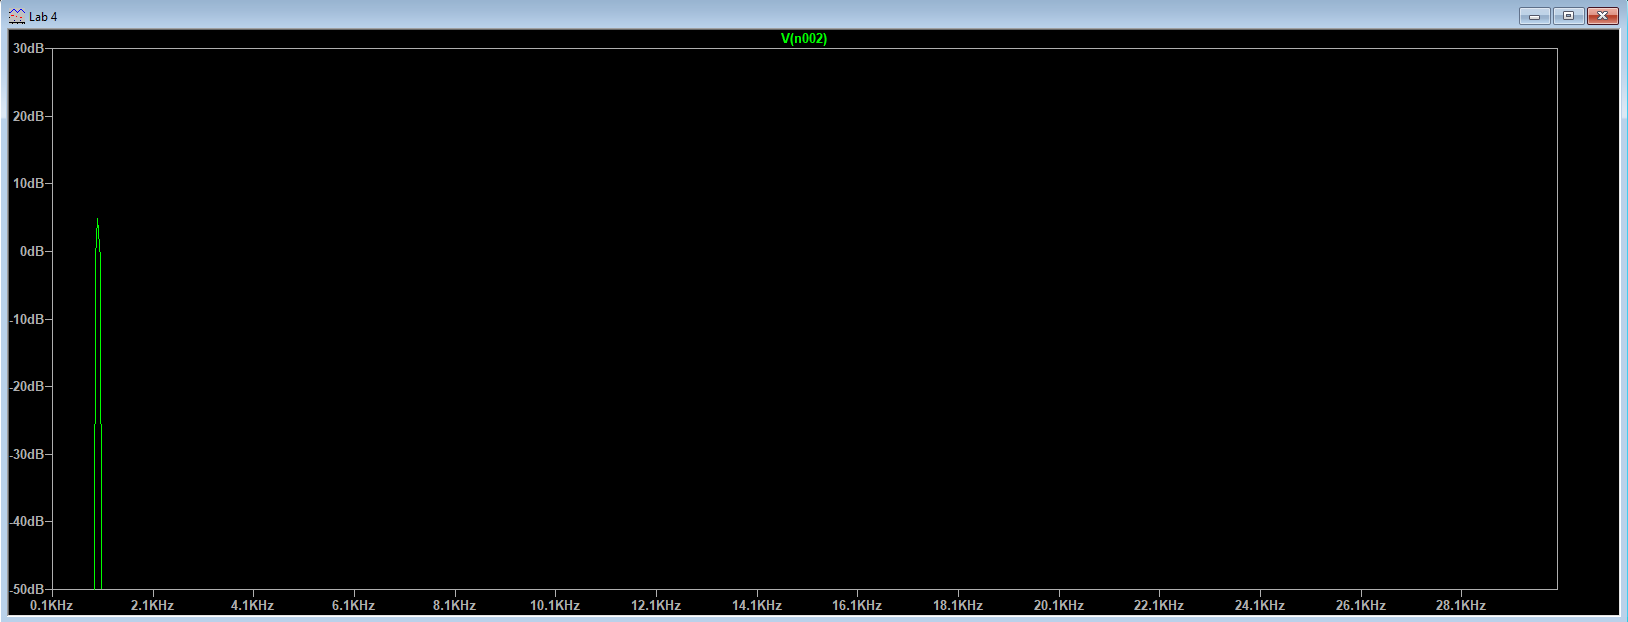
\includegraphics[width=0.75\textwidth]{Copy of Lab 4 - 2.4.PNG}
	\caption{2.4 Sinusoidal FFT}
	\label{fig:fig5}
\end{figure}

In summary, changing the source to a sinusoidal signal resulted in an FFT plot with a single frequency component at 
1000 Hz, with no harmonics or additional frequency components, highlighting the fundamental difference between the 
frequency spectra of sine waves and other periodic signals like pulses or square waves. This can be easily observed in 
Figure \ref{fig:fig5}.
\newline

\begin{figure}[H]
	\centering
	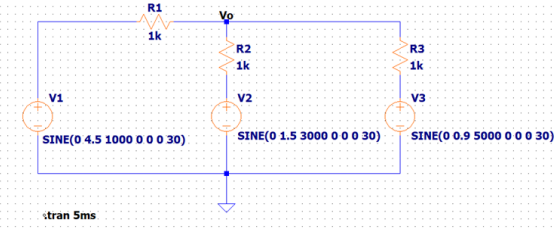
\includegraphics[width=0.5\textwidth]{26circuit.png}
	\caption{2.6 Circuit}
	\label{fig:fig6}
\end{figure}


Then a circuit (Figure \ref{fig:fig6}) with three sinusoidal voltage sources
(\(V_1\), \(V_2\), and \(V_3\)) was constructed, each operating at different
harmonic frequencies. The voltage sources were configured as follows:
\begin{itemize} \item \(V_1\) at a fundamental frequency of 1 kHz, \item \(V_2\)
at the third harmonic frequency of 3 kHz, and \item \(V_3\) at the fifth
harmonic frequency of 5 kHz. \end{itemize} The voltage at node \(V_o\) was
expressed as: \[ v_o(t) = \frac{1}{3}(v_1(t) + v_2(t) + v_3(t)), \] where each
sinusoidal voltage contributed to the overall waveform at \(V_o\).
\newline

\begin{figure}[H]
	\centering
	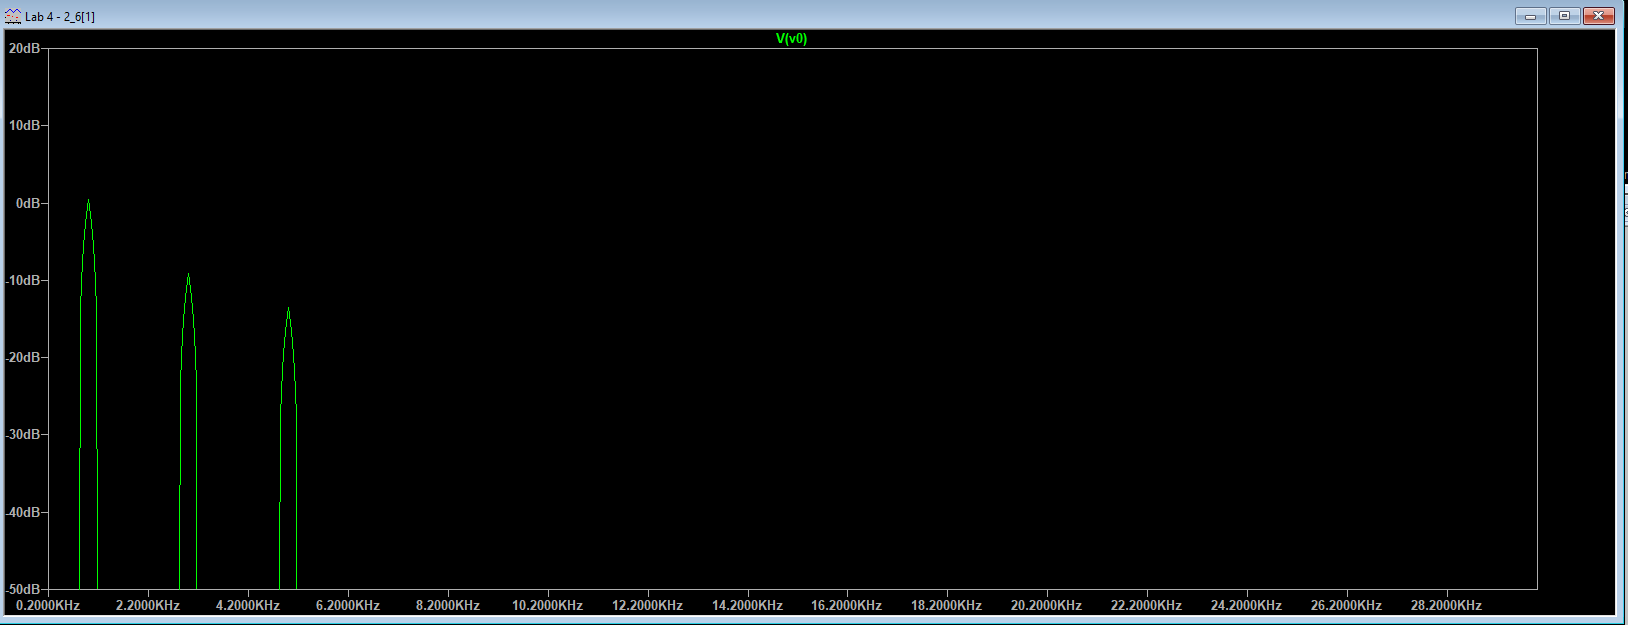
\includegraphics[width=0.75\textwidth]{Copy of Lab 4 - 2.6.PNG}
	\caption{2.6 FFT}
	\label{fig:fig7}
\end{figure}

The Fast Fourier Transform (FFT) plot in Figure \ref{fig:fig7} clearly shows distinct peaks at 
approximately 1 kHz, 3 kHz, and 5 kHz. These correspond to the fundamental frequency and its third 
and fifth harmonics, generated by the voltage sources \(V_1\), \(V_2\), and \(V_3\) respectively. 
The magnitude of the FFT, displayed in decibels (dB) on the vertical axis, ranges from -50 dB to 20 dB. 
The primary peak at 1 kHz has the highest magnitude, while the peaks at 3 kHz and 5 kHz have slightly lower 
magnitudes, which is typical for harmonic analysis.
\newline

The FFT plot shows no significant energy at frequencies other than 1 kHz, 3 kHz, and 5 kHz, confirming 
that the signal at node \(V_o\) consists only of the fundamental frequency and its harmonics. This lack 
of additional peaks indicates that there is no distortion or non-harmonic frequencies present in the system.
\newline

\begin{figure}[H]
	\centering
	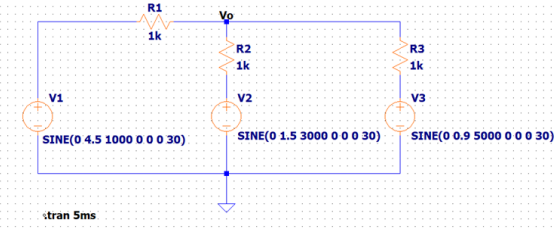
\includegraphics[width=0.5\textwidth]{26circuit.png}
	\caption{2.7 Circuit}
	\label{fig:fig8}
\end{figure}

Next, the amplitudes and phases of the voltage sources \(V_1\), \(V_2\), and \(V_3\) were modified to match Figure \ref{fig:fig8}. 
Notably, the initial phase of \(V_2\) was changed to 180°, which shifted the phase of the third harmonic relative to the fundamental 
and the fifth harmonic.
\newline

By observing the voltage \(v_o\) as a function of time, the resulting waveform showed a distinct difference 
compared to the waveform from section 2.6. The phase shift of \(V_2\) caused destructive interference between 
the harmonics, significantly altering the overall shape of the waveform. Specifically, the third harmonic (3 kHz) 
being out of phase with the fundamental (1 kHz) and the fifth harmonic (5 kHz) led to a waveform with more flattened 
or distorted peaks and troughs. This flattening effect is due to the cancellation of certain frequency components, 
reducing the constructive interference that was present in section 2.6.
\newline

\begin{figure}[H]
	\centering
	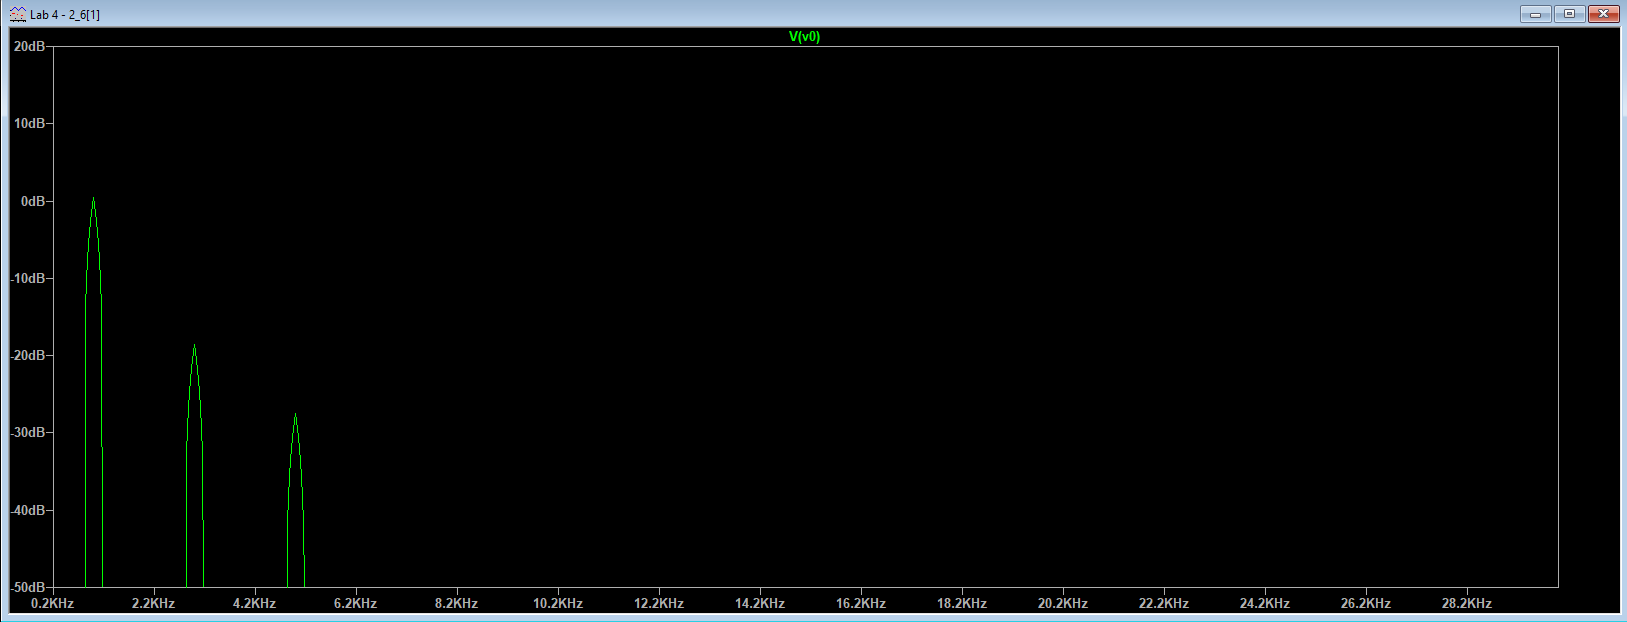
\includegraphics[width=0.75\textwidth]{Copy of Lab 4 - 2.7.PNG}
	\caption{2.7 FFT}
	\label{fig:fig9}
\end{figure}


In section 2.6, where all the harmonics were in phase, the constructive interference between the fundamental 
and its harmonics created a more regular and symmetric waveform, with sharp peaks and pronounced troughs. 
In contrast, the waveform in section 2.7 (Figure \ref{fig:fig9}) demonstrated a reduction in peak amplitude and a more flattened appearance,
 particularly at points where the fundamental and harmonics would have otherwise reinforced each other.
\newline

This comparison highlights the relationship between harmonic amplitudes and the shape of the waveform. 
When the harmonics are in phase, their amplitudes add constructively, resulting in sharper waveform variations. 
However, when harmonics are out of phase, as seen with the phase-shifted third harmonic in section 2.7, destructive 
interference occurs, flattening the waveform and reducing its amplitude at specific points.
\newline

This experiment demonstrates that the phase relationships and relative amplitudes of harmonic components are 
crucial in determining the overall waveform shape. Altering the phase of just one harmonic can significantly 
impact both the time-domain representation and the corresponding frequency content.
\newline




In this part of the lab, the resistor \(R_2\) in Figure \ref{fig:fig2} was replaced with a 1 microfarad capacitor, 
and the analysis from part 2.2 was repeated using a square wave source. The primary objective was to observe 
how the Fourier components of the input voltage (square wave) compared to those across the capacitor (output voltage), 
particularly by examining the impact of the capacitor on the signal's frequency content.
\newline\

The input signal, a square wave, is rich in harmonic content, containing not just the fundamental frequency but 
also a series of odd harmonics (third, fifth, seventh, etc.). This was evident in the FFT plot of the input signal, 
which showed distinct peaks at the fundamental frequency and its odd harmonics, with decreasing magnitudes at higher frequencies.
\newline

\begin{figure}[H]
	\centering
	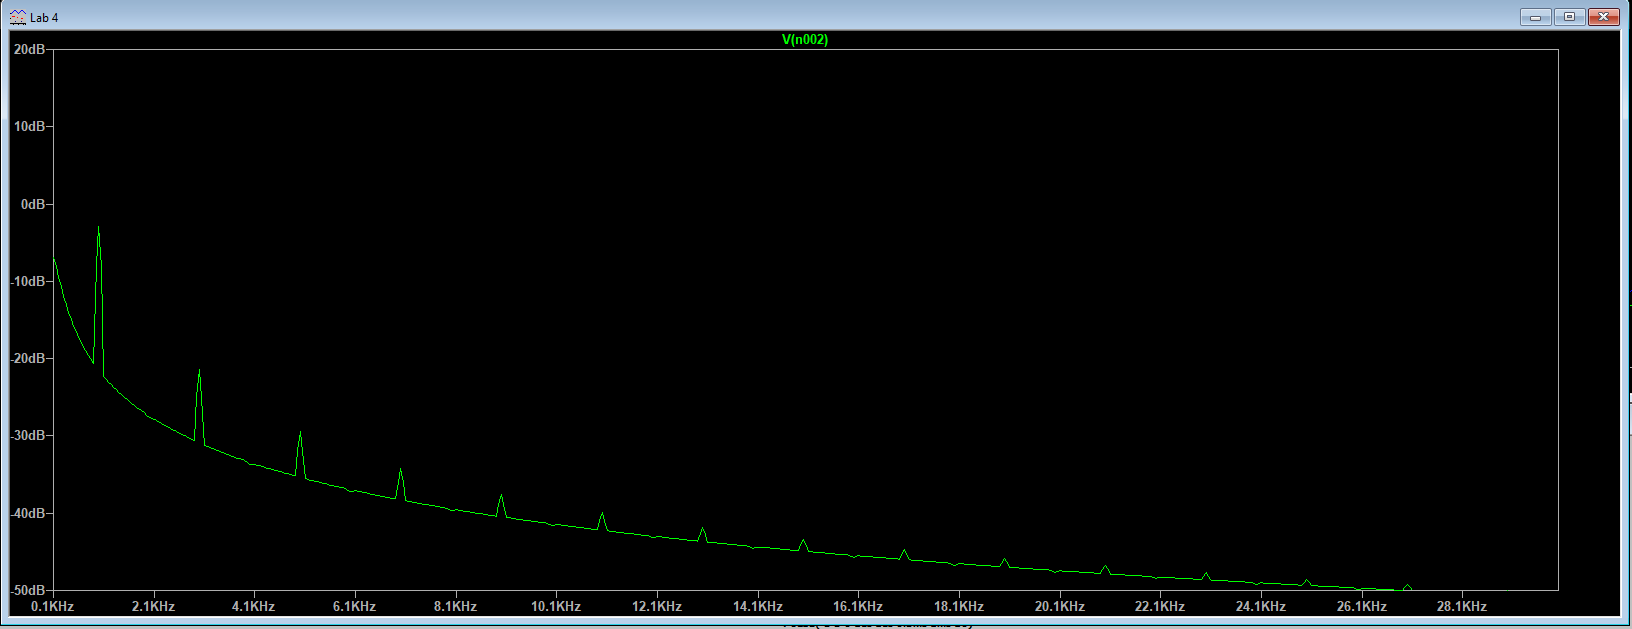
\includegraphics[width=0.75\textwidth]{Copy of Lab 4 - 2.8.PNG}
	\caption{2.8 FFT}
	\label{fig:fig10}
\end{figure}

When the resistor was replaced with a capacitor, the output voltage across the capacitor behaved differently 
due to the frequency-dependent nature of capacitive reactance. Specifically, the reactance of a capacitor decreases 
as frequency increases, meaning that higher-frequency components of the input signal (i.e., the harmonics) were more 
heavily attenuated by the capacitor. The result was a more pronounced reduction in the higher harmonics compared to the 
fundamental frequency. This can be seen in the FFT plot of the output voltage (Figure \ref{fig:fig10}), where the magnitude of the higher harmonics 
was significantly diminished compared to the input signal.
\newline

The FFT plot for the output voltage across the capacitor shows the following characteristics:
\begin{itemize}
	\item The fundamental frequency (1 kHz) remains relatively strong, but the higher harmonics are significantly attenuated, particularly beyond 3 kHz.
	\item The magnitude of the harmonics decreases rapidly, as evidenced by the steep drop-off in harmonic content beyond the third harmonic, leading to a much smoother frequency response compared to the input.
	\item The capacitor effectively acts as a low-pass filter, allowing the fundamental frequency to pass through while reducing the higher-frequency harmonics.
\end{itemize}


Replacing the resistor \(R_2\) with a capacitor altered the frequency response of the circuit, significantly 
attenuating the higher harmonics of the square wave input. The capacitor's low-pass filtering effect was clearly 
observed in the FFT analysis, where the higher-frequency components of the signal were greatly reduced, leaving 
the fundamental frequency and a small number of lower harmonics. This demonstrates the effect of capacitive reactance 
on periodic signals, particularly its role in filtering out high-frequency components.



\section{Discussions and Conclusions}
This lab successfully demonstrated the fundamental principles of signals and frequency components 
through both experimental and simulation-based methods. By using oscilloscopes and function generators, 
different waveforms, including sinusoidal, square, and ramp waves, were analyzed in the time domain. The 
study revealed that waveform shape, frequency, and amplitude directly influence both the visual signal on the 
oscilloscope and the auditory perception when applied to a speaker. Additionally, the analysis highlighted the 
limitations of human hearing, as our ability to perceive frequencies diminishes as we approach the lower and upper 
limits of the human hearing range.
\newline

Through the use of LTSpice, Fourier and transient analysis were performed, allowing for a deeper understanding of the 
frequency content of signals. It was evident that non-sinusoidal waveforms contain significant harmonic components, 
while sinusoidal signals are composed only of the fundamental frequency. This was demonstrated clearly by the FFT plots, 
which showed peaks at harmonic frequencies for square and pulse waves, and a single peak for pure sine waves.
\newline

Moreover, the experiment with altering the pulse width and phase of harmonic components further illustrated how these 
factors influence the shape and harmonic content of signals. The phase shift in one harmonic produced noticeable changes 
in the waveform, demonstrating the importance of phase and amplitude relationships in waveform composition.
\newline

Finally, the replacement of a resistor with a capacitor in the circuit demonstrated the filtering effect of capacitive 
reactance. The FFT analysis showed that higher-frequency components were attenuated, confirming the role of the capacitor 
as a low-pass filter.
\newline

Overall, this lab provided valuable insights into the behavior of signals, the importance of harmonics, and how circuit 
components such as capacitors influence signal frequency. The skills developed in using oscilloscopes, function generators, 
and LTSpice will serve as a foundation for more complex signal processing tasks in future studies.
\newline

\section{References}
 [1] Dr. Iman Salama. “Lab 4 – Basics of Signals: Frequency” Northeastern University. 4 October 2024.

\end{document}
